\documentclass[a4paper,12pt,times,numbered,print,index]{article}

\usepackage[italian]{babel}
\usepackage[utf8]{inputenc}
\usepackage{graphicx}
\usepackage{listings}
\usepackage{color}
\usepackage{fancyhdr}
\usepackage[margin=1in]{geometry}
\usepackage{hyperref}
\usepackage[backend=biber, style=authortitle-comp]{biblatex}
%
% File della bibliografia
%
\addbibresource{bibliografia.bib}

%
% Impostazioni per head e foot
%
\pagestyle{fancy}
\fancyhead{}
\fancyfoot{}
\fancyhead[R]{Designer}
\fancyfoot[L]{\thepage}
\fancyfoot[R]{\slshape{\footnotesize{Guglielmo Bartelloni - Francesco Bellezza}}}

%
% Impostazioni per link dell'indice
%
\hypersetup{
    colorlinks,
    citecolor=black,
    filecolor=black,
    linkcolor=black,
    urlcolor=black
}

% Colori per inserire syntax highlight
\definecolor{dkgreen}{rgb}{0,0.6,0}
\definecolor{gray}{rgb}{0.5,0.5,0.5}
\definecolor{mauve}{rgb}{0.58,0,0.82}

% Setting per Java

\lstset{frame=tb,
  language=Java,
  aboveskip=3mm,
  belowskip=3mm,
  showstringspaces=false,
  columns=flexible,
  basicstyle={\small\ttfamily},
  numbers=none,
  numberstyle=\tiny\color{gray},
  keywordstyle=\color{blue},
  commentstyle=\color{dkgreen},
  stringstyle=\color{mauve},
  breaklines=true,
  breakatwhitespace=true,
  tabsize=3
}
\author{Guglielmo Bartelloni}
%
% Inizio del documento
%
\begin{document}
%
% TITOLO
%
\begin{titlepage}
\begin{center}
	\vspace{1cm}
	\textbf{\huge{Designer}}\\ 
	\vspace{1cm}
	
\includegraphics[scale=0.7]{logoITTS.jpg}\\
	\vspace{1cm}
	\large{Guglielmo Bartelloni, Francesco Bellezza}\\
	\vspace{0.5cm}
	24 Dicembre, 2017\\
	\today\\
	\vspace{0.5cm}
	\vspace{0.5cm}
	4IB\\
	Luigi Vestri e Davide Caramelli\\
	\vspace{1cm}
	\Large{Laboratorio di Informatica}
\end{center}
\end{titlepage}
\vspace*{1cm}
\tableofcontents
\clearpage
%
% Inizio del CORPO
%
\section{Scopo dell'esercitazione}
Lo scopo dell'esercitazione e quella di realizzare un programma che consenta di disegnare figure geometriche e grafici di funzioni permettendo di salvare le figure sul un file di testo.

\section{Cenni Storici}


\subsection{Ereditarieta'}
L’ereditarietà è una relazione di tipo is-A, dove una superclasse mette a disposizione di una sottoclasse i suoi metodi e attributi non privati (a eccezione del costruttore).

In Java, per estendere una superclasse e per creare quindi la sottoclasse, si utilizza la parole chiave extends accanto al nome della sottoclasse e accanto alla parola extends si inserisce il nome della superclasse.

Nel caso delle interfacce, ovvero particolari classi che al loro interno contengono solamente metodi astratti, si utilizza la parola chiave implements.
\textcite{corsoinformatica}

\subsection{Polimorfismo}
Il polimorfismo è una tecnica che consente di utilizzare metodi polimorfici, ovvero metodi che hanno lo stesso nome, ma implementazioni diverse.
Esistono due tipi di polimorfismi principali: per overloading e per overriding.

Nel polimorfismo per overloading si opera a un livello locale, ovvero all’interno di una classe.

Il metodo polimorfico in questo caso deve:
\begin{itemize}
	\item Avere lo stesso nome degli altri metodi polimorfici.
	\item Avere numero di parametri diversi o avere tipi di parametri diversi o avere ordine di parametri diversi rispetto agli altri metodi polimorfici.
	\item Può avere un tipo di ritorno diverso se i due punti qua sopra sono rispettati.
\end{itemize}
Nel polimorfismo per overriding si opera a un livello di superclassi e sottoclassi.

Nelle sottoclassi viene ridefinito il metodo presente nelle superclassi.

Il metodo polimorfico in questo caso deve:
\begin{itemize}
	\item Avere la stessa signature del metodo della superclasse.
	\item Avere lo stesso tipo di ritorno della superclasse o un sottotipo del tipo di ritorno della superclasse (stesso discorso vale per i parametri).
	\item I metodi private non vengono ereditati alla classe figlia, quindi non si può effettuare l’overriding del metodo.
	\item Le clausole come native, strictfp possono essere incluse nel metodo della classe figlia.
	\item Un metodo statico può essere solo adombrato e non sovrascritto.
\end{itemize}
\textcite{polimorfismo}


\section{Analisi Funzionale}


\subsection{Ipotesi Risolutiva}
Il programma deve riuscire a disegnare figure elementari su un pannello. Per farlo viene utilizzato l`oggetto graphics andando a reimplementare la classe 
\begin{lstlisting}
public void paintComponent(Graphics g);
\end{lstlisting}

\subsection{Funzionalitá del programma}
Le funzionalitá che si devono implementare sono:
\begin{enumerate}
	\item Salvare su file
	\item Caricare da file
	\item Disegnare figure(quadrato, arco, linea, ellisse, rettangolo, grafico, cerchio e ellisse)
	\item Disegnare Font(grandezza, tipo,  stile)
\end{enumerate}


L`interfaccia si presenta in questo modo:


\section{Analisi Tecnica}

\subsection{Scomposizione Top-Down} \label{TopDown}
La scomposizione Top-Down del Main é la seguente:
\begin{lstlisting}
	INIZIO
		imposta le dimensioni del frame
		inizializza le icone
		crea i componenti della GUI
		aggiungi i listener
		imposta la finestra non ridimensionabile
	FINE
\end{lstlisting}
\subsection{UML}
\begin{center}
	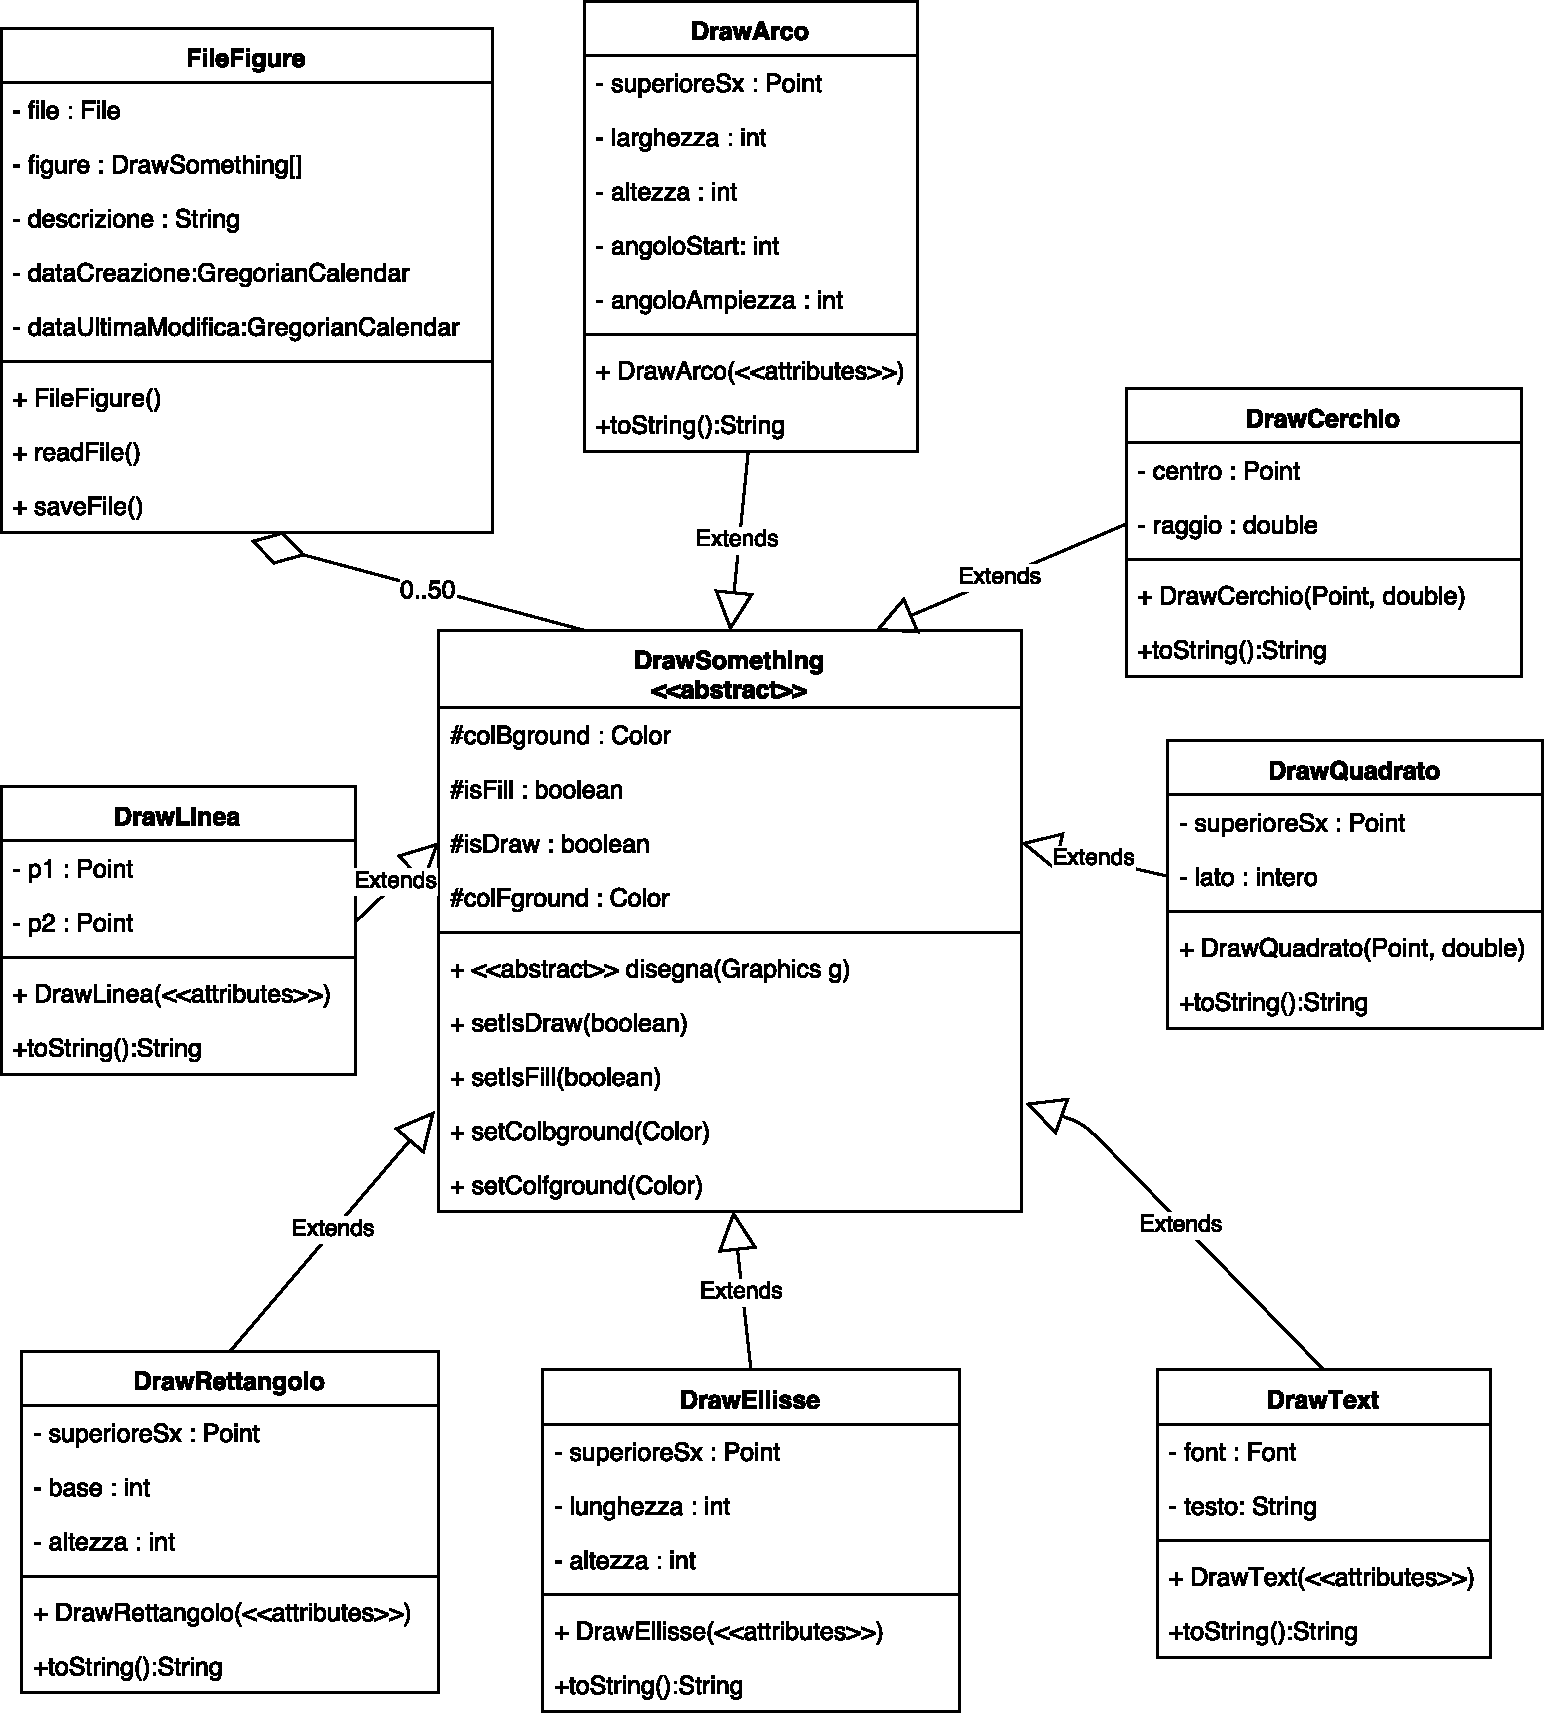
\includegraphics[scale=0.4]{Immagini/UML.pdf}
	\label{UML}
\end{center}


\subsection{Descrizione Classi}
Le classi del programma Designer sono divise per package a seconda del loro utilizzo all'interno del programma stesso, essi sono:
\begin{itemize}
	\item \textit{File}: contiene le classi che si occupano della gestione dei file.
	\item \textit{GUI}: contiene le classi che si occupano della gestione della grafica insieme alle classi che rappresentano le varie Dialog e la tabella.
	\item \textit{Grafico}: contiene la classe Funzione che rappresenta una funzione matematica.
	\item \textit{UtilitiesForDrawing}: contiene le classi che si occupano del disegno delle figure geometriche compreso anche il grafico della funzione e il font.
	\item \textit{VectorAndException}: contiene la classe che rappresenta il vettore di figure insieme alle eccezioni ad esso collegate.
	\item \textit{icons}: contiene tutte le immagini delle icone utilizzate.
	\item \textit{lookAndFeel}: contiene i .jar del Look And Feel utilizzato.
\end{itemize}
Di seguito verranno descritte solo le classi principali.
\subsubsection{MainFrame} %Nome della classe
La classe \textit{MainFrame} è la classe che si occupa di gestire tutti gli oggetti del programma, infatti rappresenta il \textit{controller} e la \textit{vista} del Design Pattern MVC. Le sue funzioni principali sono state esplicitate in \ref{TopDown}. La classe è stata scomposta in molti sottometodi per facilitare la lettura e la scrittura. Viene implementato il MouseListener registrato sul \textit{pnlDisegno} e nel momento in cui l'utente preme sul pannello viene registrata la posizione (iniziale) del mouse poi, al rilascio, viene registrata la posizione (finale) del mouse inizializzando e inserendo nel vettoreFigure la figure precedentemente selezionata dall'utente.

\textit{setSelectedBotton()} è un particolare metodo per riuscire a lasciare selezionati i pulsanti delle figure e dello stile dei font, semplicemente deseleziona tutti i pulsanti che non corrispondono a quello premuto.

Al rilascio del pulsante del mouse vengono fatti vari controlli delle coordinate per farsì che la figura sia disegnata correttamente: se per esempio l'utente trascina da in alto a sinistra fino in basso a sinistra dovranno essere scambiate le coordinate come segue
\begin{lstlisting}
  pInf.setLocation(pIniziale.x, pFinale.y);
  pSup.setLocation(pFinale.x, pIniziale.y);
  pIniziale.setLocation(pSup);
  pFinale.setLocation(pInf);
\end{lstlisting}
Al suo interno è presente una inner class, che ha come scopo quello di gestire il \textit{JMenuBar} e di gestire la creazione di un file, il caricamento e il salvataggio.

\subsubsection{DrawSomething}
La classe \textit{DrawSomething} é una classe astratta che dichiara alcuni metodi per impostare i colori e un metodo astratto per essere riscritto nelle classi figlie.
É pensata all'unico scopo di essere estesa dalle altre classi \textit{draw} che implementeranno il metodo \textit{toString()} e il metodo \textit{draw(Graphics g)} come mostrato in figura \ref{UML}.
Gli attributi di questa classe sono i seguenti:
\begin{lstlisting}
protected Color colBground;
protected Color colFground;
\end{lstlisting}

\subsubsection{FileFigure}
La classe \textit{FileFigure} é la classe che si occupa di gestire di gestire il ripristino e il salvataggio delle figure nel file di testo.
Un file di testo, per essere letto, deve avere al suo interno:
\begin{enumerate}
\item Descrizione
\item Data Creazione
\item Data Ultima Modifica
\item Colore sfondo
\item Figure da disegnare
\end{enumerate}
Al suo interno sono presenti i seguenti metodi:

Il metodo \textit{setWrittable()} serve per creare una istanza della classe PrintWriter che scrive sul file. Se la funzione ritorna un valore uguale a \textcolor{blue}{false}, allora c'è stato un qualche errore dovuto all'Input/Output.

Il metodo \textit{setReadable()} serve per creare una istanza della classe BufferedReader che legge il file. Se la funzione ritorna un valore uguale a \textcolor{blue}{false}, allora c'è stato un qualche errore dovuto all'Input/Output: ad esempio il file non è stato trovato.


Il metodo \textit{readFile()} si occupa di leggere il file di testo e salvare le figure nell'array.

Il metodo \textit{saveFile()} si occupa di salvare l'array di figure all'interno del file di testo. Per il salvataggio delle figure viene utilizzato il metodo \textit{toString()} di ogni figura.

\subsubsection{Funzione}
La classe \textit{Funzione} é una classe che rappresenta una funzione matematica contiene infatti l'insieme di coefficienti insieme al termine noto all'interno di un'array di \textit{double}.
Gli attributi di questa classe sono i seguenti:
\begin{lstlisting}
	private double[] coefficienti
\end{lstlisting}
Contiene un metodo per ottenere la \textit{y} data una \textit{x} come parametro:
\begin{lstlisting}
public double getRisultato(double x);
\end{lstlisting}
e un metodo per aggiungere i coefficienti:
\begin{lstlisting}
 public boolean add(double coefficiente, int potenzaCoef);
\end{lstlisting}

\subsubsection{Vector}
La classe \textit{Vector} é la classe che rappresenta un vettore di dimensione iniziale di 100 Object. Contiene i metodi per rendere dinamico il vettore, infatti ogni volta che verrá aggiunto un elemento ci sará un controllo che verificherá che il numero di elementi non superi la grandezza del vettore, se viene superata allora verrá lanciata l'eccezione \textit{IsFullException} che deve essere catturata per poter richiamare il metodo \textit{riorganizza()}. Il metodo \textit{riorganizza()} si occupa di ricreare l'array con dimensione doppia rispetto a quella iniziale e di immettere gli elementi al suo interno.
É presente anche un metodo per rimuovere gli elementi data una posizione facendo uno shift verso sinistra:
\begin{lstlisting}
	public void removeElement(int pos);
\end{lstlisting}
I parametri della classe sono:
\begin{lstlisting}
protected Object[] items;
protected int index;
public static int DIMENSIONE;
\end{lstlisting}

\subsubsection{VectorDraw}
Classe che estende la classe \textit{Vector} in modo da contenere elementi di tipo \textit{DrawSomething}.
Contiene due metodi che servono uno, per ritornare l'array di DrawSomething, l'altro, per ritornare la singola figure presente nella posizione data come parametro.
\subsubsection{JColorChoicePane}
Pannello che ha la funzione di visualizzare la scelta dei colori contiene un \textit{ItemListener} per salvare il colore una volto che viene scelto.
\subsubsection{JButtonColor}
La classe \textit{JButtonColor} é stata creata appositamente perché il programma utilizza un Look and Feel diverso da quello di default. Il problema che abbiamo riscontrato con questo, é che i componenti non possono essere cambiati di colore al di fuori del \textit{paintComponent(Graphics g)}. Abbiamo dovuto quindi, per la scelta del colore, creare dei bottoni che disegnino un rettangolo al loro interno con il colore selezionato dall'utente nel \textit{JColorChoicePane}.
\subsubsection{JPanelDrawing}
Rappresenta il pannello per il disegno, ovvero il foglio bianco su cui disegnare le figure. Presenta il metodo \textit{paintComponent(Graphics g)} che disegna tutte le figure del vettore attraverso un \textit{for} e richiamando il metodo \textit{draw(Graphics g)} di ogni figura.
\subsubsection{JDialogArc}
Rappresenta una \textit{Dialog} che si occupa di [rendere i dati necessari per costruire l'arco 
\subsubsection{JDialogGrafico}
Rappresenta una \textit{Dialog} che si occupa di prendere i dati necessari per la creazione del grafico. Permette di inserire i dati con un formato a matematico uno alla volta del tipo:\\
$2x^2$\\
in questo
\begin{lstlisting}
2x2
\end{lstlisting}

\section{Test Data Set/Debug}

\printbibliography
\end{document}
